\subsection{Message Queues}\label{sec:messagequeues}

\subsection{Verallgemeinerung des Erzeuger-Verbraucher-Problems}

Bei \textbf{Message Queues} bleiben Nachrichten als Einheiten erhalten (\textbf{nachrichtenorientierte Kommunikation}, bspw. \textbf{UDP}\footnote{User Datagram Protocol}).\\

\noindent
\textbf{Pipes} repräsentieren \textbf{datenstromorientierte Kommunikationsmodelle} (bspw. \textbf{TCP}\footnote{Transmission Control Protocol})  - der Empfänger sieht nicht, in welchen Portionen die Daten gesendet werden.\\

\noindent
Eine Message Queue besitzt einen \textbf{Puffer}, der entweder viele kleine oder wenig große Nachrichten entgegennehmen kann.\\

\noindent
Bei \textbf{Message Queues} werden die Nachrichten in ihrer Gesamtheit in Feldern gespeichert (bspw.~\code{byte[][]}).\\

\noindent
Bei \textbf{Pipes} werden Nachrichten in eindimensionalen Feldern (bspw.~\code{byte[]}) gespeichert (in zyklischer Weise) - dadurch sind Nachrichtengrenzen nicht zu erkennen.\\

\noindent
Das Senden bei Pipes erfolgt i.d.R. als unteilbare Aktion.
\begin{itemize}
    \item Wenn die Nachricht größer ist als der \ul{im Puffer verbleibende Platz}, wird gewartet, bis der Platz frei ist - dann wird \textbf{auf einen Schlag} in den Puffer kopiert
    \item Ist die Nachricht länger als \ul{die Größe des Puffers}, wird die Nachricht geteilt und in Portionen gesendet - dadurch kann es vorkommen, dass Nachrichtenteile durchgemischt werden; sind die Nachrichtenteile nicht größer als die Pufferlänge, befinden sie sich komplett im Puffer;  umgekehrt ist es möglich, dass Stücke von Nachrichtenteilen ``durchgemischt`` werden (vgl.~\cite[117 f.]{Oec22}).
\end{itemize}

Beim Empfangen wird nur so lange gewartet, bis der Puffer nicht mehr leer ist:
\begin{itemize}
    \item der Empfänger gibt an, wie viele Bytes ($n$) er lesen möchte.
    \item ist der Puffer komplett leer, wird mit dem Lesen gewartet, bis Daten im Puffer sind.
    \item Es werden $n$ Daten aus dem Puffer gelesen - sind weniger als $n$ Daten im Puffer, werden auch nur soviele Daten gelesen (die Daten werden hierbei in ein Feld passender Länge kopiert).
\end{itemize}

\subsection{Das Philosophen-Problem}
 Das \textbf{Philosophen-Problem}\footnote{
Wikipedia - Dining Philosophers Problem: \url{https://en.wikipedia.org/wiki/Dining_philosophers_problem} - abgerufen 27.01.2024
}
veranschaulicht die Entstehung von Verklemmungen: An einem runden Tisch sitzen 5 Philosophen ($P_1,...,P_5$), die abwechselnd mit Denken und Essen beschäftigt sind (s. Abbildung~\ref{fig:philosopher}).\\
\noindent
 Zum Essen benötigen die Philosophen Gabeln, und zwar eine in jeder Hand.
 Die Gabeln liegen genau zwischen den Philosophen.
 Angenommen, alle Philosophen sind mit Denken beschäftigt.
 Wenn jetzt ein Philosoph $P_1$ davon zum Essen übergeht, greift er links eine Gabel, und genau in dem Moment wollen die anderen Philosophen auch zum Essen übergehen: Alle nehmen ihre linken Gabeln.
$P_1$ möchte nun die rechte Gabel nehmen, die aber als linke Gabel von $P_5$ von diesem gehalten wird - also muss $P_1$ warten, bis $P_5$ seine Gabel freigibt - der gleichzeitig aber nicht essen kann, weil er dazu die Gabel benötigt, die $P_4$ hält.
Da alle Philosophen auf eine Freigabe der Gabeln warten, kommt keiner dazu, zu essen.

\begin{figure}
    \centering
    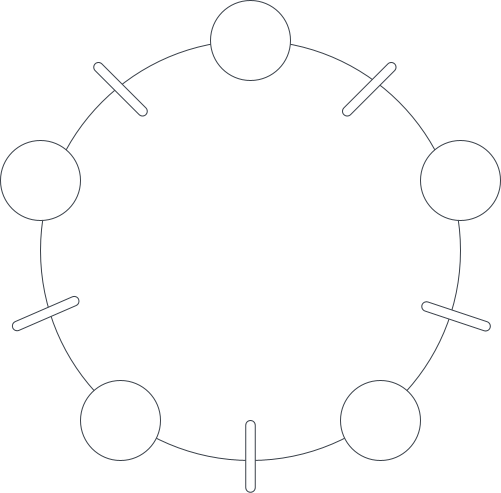
\includegraphics[scale=0.25]{chapters/fopt2/img/philosopher}
    \caption{ Eine Illustration des Philosophen-Problems: Ein Philosoph benötigt jeweils die Gabel links und rechts von ihm zum Essen (Quelle: eigene)}
    \label{fig:philosopher}
\end{figure}

\noindent
Diese Verklemmungssituation läßt sich bspw. durch Semaphorgruppen lösen, wobei ein Philosoph jeweils zwei Gabeln \textbf{auf einen Schlag} anfordert, oder auch durch $n$ Semaphore, wobei jeder Semaphor eine Gabel repräsentiert, und ein zusätzlicher Semaphor als ``Essenserlaubnis``, die den ``Gabel-Semaphoren`` vorgeschaltet ist, wie im folgenden Beispiel:

\begin{minted}[mathescape,
    linenos,
    numbersep=5pt,
    gobble=2,
    fontsize=\small,
    frame=lines,
    framesep=2mm]{java}
    public void run() {
        while (true) {
            // eatLock ist eine Mutex-Semaphore.
            // left() und right() rufen jeweils p()
            // (bzw. v() wenn release == true) auf
            // die benachbarten Gabeln auf (wobei Gabel rechts ==
            // index des aufrufenden Philosophen ist)
            eatLock.acquire();
            table.left(position, false).right(position, false);
            eatLock.release();

            table.left(position, true).right(position, true);
        }
\end{minted}\\



\subsection{Leser-Schreiber-Problem}\label{subsec:readerwriterproblem}

\textbf{Leser-Schreiber-Problem}: Es soll lesen erlaubt sein von beliebig vielen Threads, aber die Änderung des Objekts durch schreibende Zugriffe darf nur von einem Thread aus geschehen.\\

\noindent
Wenn alle Zugriffe \textbf{synchron} sein müssen, würde das Objekt beim Lesen als auch beim Schreiben blockiert - das schränkt die Parallelität ein, vor allem, wenn der Lesevorgang länger dauert und das Objekt somit nicht aktualisiert werden kann.\\

\noindent
$\rightarrow$ Es muss eine Lösung gefunden werden, so dass mehrere Threads lesen, aber nur ein Thread schreiben kann.\\

\noindent
Zur Lösung sind verschiedene Strategien denkbar:

\begin{itemize}
    \item \textbf{Bevorzugung der Leser}, falls es darauf ankommt, dass die Leser schnell Zugriff auf die Daten erhalten, und die Aktualität der Daten weniger wichtig ist
    \item \textbf{Bevorzugung der Schreiber}, falls die Aktualität der Daten wichtiger ist
\end{itemize}\\

\noindent
Die Strategien können nur dann sinnvoll eingesetzt werden, falls kein Thread unerwünscht lange auf seinen Zugriff warten muss.\\
Kann eine gewisse Wartezeit für Leser/Schreiber nicht garantiert werden, bietet sich eine strengere Strategie an: Zugriffswünsche landen in einer Warteschlange, immer der zuerst eingefügte wird abgearbeitet (\textbf{FIFO}).


\subsection{Schablonen zur Nutzung der Synchronisationsprimitive und Konsistenzbetrachtungen}

Der \textbf{Zustand} eines Objektes wird durch die Werte seiner Attribute beschrieben.\\

\noindent
Gewisse Konsistenzbedingungen\footnote{bestimmte Invarianten bzw. Integritätsbedingungen} gelten für manche solcher Attribute immer $\rightarrow$ das Ändern solcher Attribute führt ein Objekt von einen konsistenten Zustand in einen anderen\footnote{
Konsistenzbedingungen können währen der Überführung eines Objektes in einen anderen Zustand verletzt werden, weshalb man bspw. Zugriffsmodifizierer wie \textit{private} verwendet.
}.\\

\noindent
Wenn mehrere Threads schreibend auf ein Objekt zugreifen, muss die durchgehende Konsistenz des Objektes gewährleistet sein, jeder Thread muss immer ein Objekt vorfinden, für das die Konsistenzbedingungen gelten.\\

\noindent
In einigen Fällen ist die Änderung des Zustands an eine bestimmte Bedingung geknüpft, die als \textbf{Wartebedingung} überprüft werden kann - diese Bedingung sollte in einer \code{while}-Schleife als Ausdruck verwendet werden, damit die Bedingung nach Freigabe erneut überprüft werden kann (sie kann zwischenzeitlich wieder geändert worden sein).\\

\noindent
Wenn nach einer Zustandsänderung wartende Threads weiterlaufen können, sollten diese im Anschluss mittels \code{notify()}/\code{notifyAll()} wieder geweckt werden - je nach Implementierung unterscheidet sich das aber, bspw. wenn \textbf{Additive Semaphore} genutzt werden: Die Zustandsänderung des Zählers bewirkt nicht gleich für alle Threads ein weiterlaufen.\\

\noindent
Komplexe Wartebedingungen implementiert man in einer eigenen Methode.\\

\noindent
Jede Methode einer Klasse (die öffentlich ist) muss sicherstellen, dass das Objekt nach Verlassen der Methode wieder in einem konsistenten Zustand ist.\\

\noindent
Exceptions sollten nicht zu einem inkonsistenten Zustand führen. Hier sollte \code{finally} zur Wahrung der Konsistenz genutzt werden.

\blockquote[{\cite[142]{Oec22}}]{
Es ist darauf zu achten, dass nach der Initialisierung und bei jeder Freigabe einer Sperre der Objektzustand konsistent ist, denn dann kann man davon ausgehen, dass der Zustand auch bei jedem Setzen einer Sperre konsistent ist.
}

\noindent
Weiter stellt \cite[138 ff.]{Oec22} 6 Schablonen vor, die für verschiedene Kategorien von \code{synchronized}-Methoden verwendet werden können:

\begin{itemize}
    \item lesende Methoden ohne \code{wait()}
    \item lesende Methoden mit \code{wait()}
    \item schreibende Methoden ohne \code{wait()} und ohne \code{notify()}/\code{notifyAll()}
    \item schreibende Methoden mit \code{wait()}, aber ohne \code{notify()}/\code{notifyAll()}
    \item schreibende Methoden ohne \code{wait()}, aber mit \code{notify()}/\code{notifyAll()}
    \item schreibende Methoden mit \code{wait()} und mit \code{notify()}/\code{notifyAll()}
\end{itemize}
